\documentclass[a4paper,11pt]{article}
\usepackage[utf8]{inputenc}
\usepackage[T1]{fontenc}
\usepackage{lmodern}
\usepackage[babel=true]{microtype}
\usepackage[portuguese]{babel}
\usepackage{graphicx}
\usepackage{color}
\usepackage{listingsutf8}
\usepackage{array}
\usepackage{tabulary}
\usepackage{float}
\usepackage{csvsimple}
\usepackage{changepage}
\usepackage[letterpaper,margin=1in]{geometry}
\lstset{
 breaklines=true,
 tabsize=4,
 inputencoding=utf8/latin1,
 columns=flexible,
 keepspaces=true
}

\begin{document}

\begin{titlepage}
\title{\huge \textbf{SQL3 ASSIGNMENT 
\\[1cm]
\includegraphics{logo.png}\\[1cm] \large Tecnologias de Bases de Dados\\[0.25cm] \small $4^o$ ano $2^o$ semestre\\[0.05cm]Mestrado Integrado em Engenharia Informática e Computação\\[1.7cm]}}

\author{Hugo Drumond \\ Rui Gonçalves \and 201102900\\ 201201775 \and up201102900@fe.up.pt \\ up201201775@fe.up.pt \\[1cm]}
\date{}
\maketitle
\thispagestyle{empty} % titlepage must not be numbered
\end{titlepage}

%\newpage
%\tableofcontents
\newpage

\section{Design an object-relational data model for this situation, exploiting the SQL3 extensions}

\subsection{Diagrama de classes uml}
Este diagrama descreve a estrutura high-level do problema. Foram acrescentadas restrições, informação de tipos e ids. Os ids podem ou não representar chaves primárias. Tal acontece na nossa transformação para o modelo relacional. No caso do modelo objeto-relacional usamos o id como identificador único para os items poderem ser encontrados facilmente numa página web, por exemplo: /clients/1, /images/1, /**/:id. 

\begin{figure}[H]
	\centering
		\noindent\makebox[\textwidth]{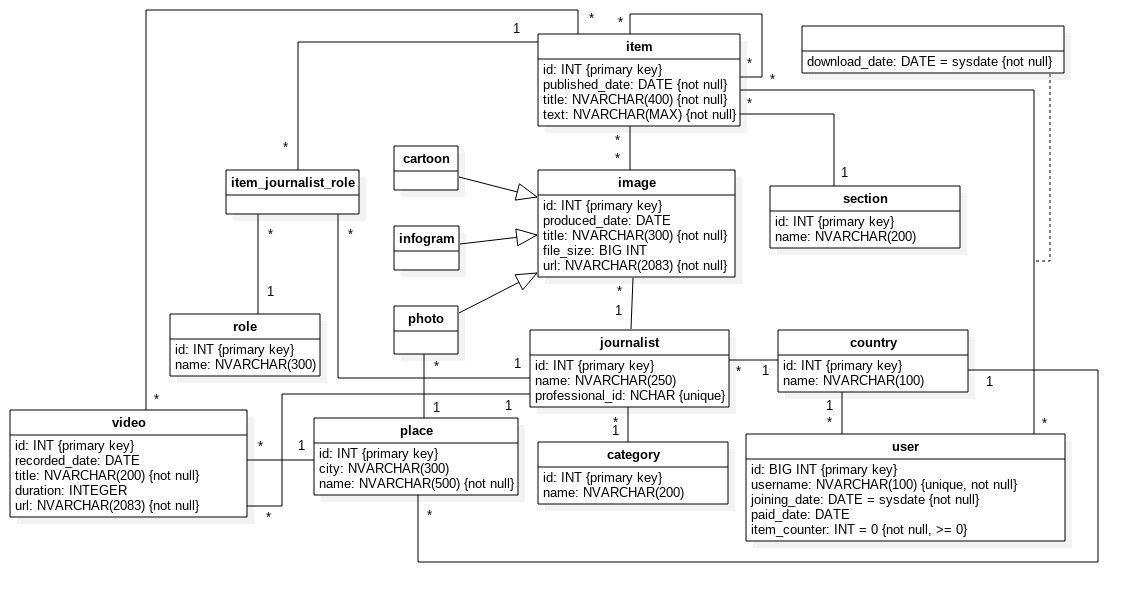
\includegraphics[width=1.2\textwidth]{../relationalClassDiagram.png}}
    \caption{Uml Class Diagram}
\end{figure}

\subsection{Modelo Relacional}
\lstinputlisting{../relational_model.txt}

\subsection{Modelo Objeto-Relacional}
\subsubsection{Esquema}
\begin{figure}[H]
	\centering
    	\noindent\makebox[\textwidth]{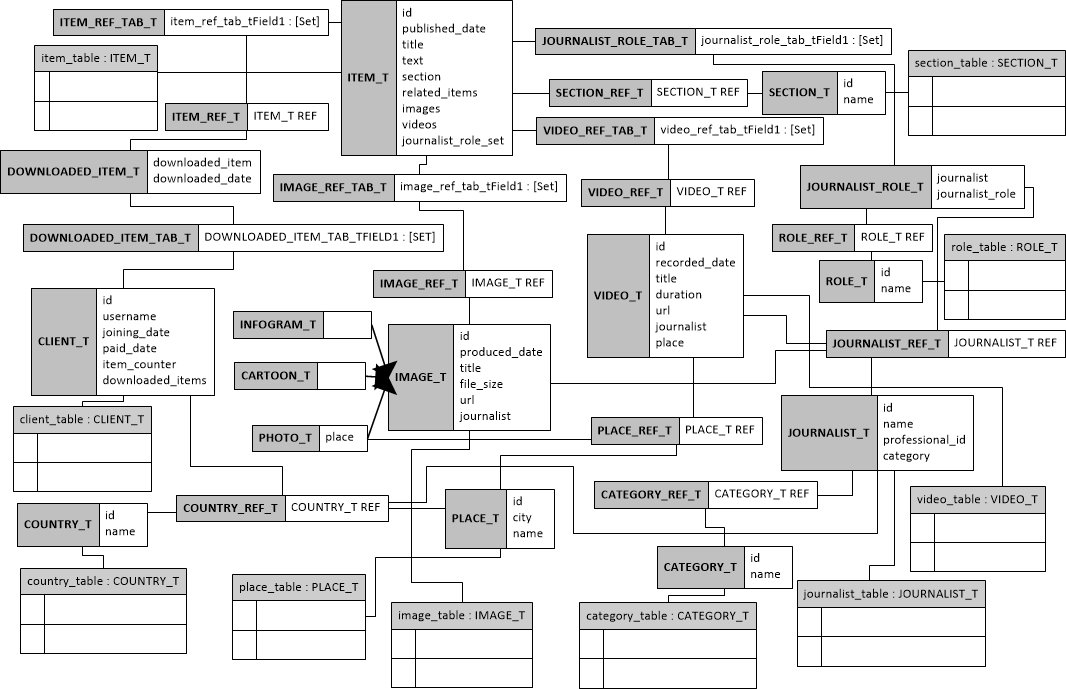
\includegraphics[width=1.2\textwidth]{../objectRelationalModel.jpg}}
    \caption{Uml Class Diagram}
\end{figure}

\subsubsection{Implementação}
\lstinputlisting[language=SQL]{../schema.sql}

\section{Prepare an instance for the DB}
\lstinputlisting[language=SQL]{../inserts.sql}

\section{Add an ordering method for the news base on descending date and, for each day, on the number of previous downloads, also descending}
\lstinputlisting[language=SQL]{../c.sql}

\section{Prepare a query that, given the reader and a day presents the titles of the photos he has seen}
\lstinputlisting[language=SQL]{../d.sql}
\begin{center}\noindent\makebox[\textwidth]{\csvautotabular[respect all]{../d.csv}}\end{center}

\section{List the production of each journalist, including statistics}
\lstinputlisting[language=SQL]{../e-views.sql}

\lstinputlisting[language=SQL]{../e1.sql}
\begin{center}\noindent\makebox[\textwidth]{\csvautotabular[respect all]{../e1.csv}}\end{center}

\lstinputlisting[language=SQL]{../e2.sql}
\begin{center}\noindent\makebox[\textwidth]{\csvautotabular[respect all]{../e2.csv}}\end{center}

\lstinputlisting[language=SQL]{../e3.sql}
\begin{center}\noindent\makebox[\textwidth]{\csvautotabular[respect all]{../e3.csv}}\end{center}

\lstinputlisting[language=SQL]{../e4.sql}
\begin{center}\noindent\makebox[\textwidth]{\csvautotabular[respect all]{../e4.csv}}\end{center}

\lstinputlisting[language=SQL]{../e5.sql}
\begin{center}\noindent\makebox[\textwidth]{\csvautotabular[respect all]{../e5.csv}}\end{center}

\end{document}
